\documentclass[preprint]{aastex}
\usepackage{amsmath,amssymb}
\usepackage{mathrsfs}
\usepackage{graphicx}
\usepackage{natbib}
\usepackage{bm}
\bibliographystyle{apj}

\newcommand{\mli}[1]{\mathit{#1}}
%\usepackage{epstopdf}

\begin{document}

\title{Model for DES Type Ia Supernova Cosmology Analysis}
\author{Alex Kim}

\section{Model}
We infer a Hubble diagram based on measurements of discovered transients
that have passed some selection criteria (e.g.\ classified as Type~Ia supernovae).  The posterior
of the Hubble diagram is denoted as
\begin{equation}
p({\mu},{z} |  {{ADU}}, {{T}}_S,{{z}}_S,
{{\theta}}_S, \theta_G, \tau).
\label{hd:eqn}
\end{equation}
The set of distance moduli
and redshifts $(\mu, z)$ contains the points that constitute the Hubble diagram.  The
data
from which the Hubble diagram is inferred include:
the transient photometry ${ADU}$; spectral measurements of
transient
type, redshift and SN-parameters ${T}_S$, ${z}_S$, ${\theta}_S$;
host-galaxy parameter measurements $\theta_H$ (including redshift,
mass, sSFR, etc.).  
The subset transients that enter the cosmology
analysis is based on the sample-selection criteria $\tau$: for example
the classification score from PSNID (a classifier based on multi-band
light curves).

The posterior of $\mu$ and $z$ is an efficient way
to distribute supernova results in is a way that is independent of cosmological model,
facilitating joint-probe analysis or consideration of non-standard models.  Choosing
a specific cosmological model, the posterior of the model parameters $\theta_\mu$
is of interest.  The model presented here accommodates both options.

A sketch of a more extensive model that includes the
model of Equation~\ref{hd:eqn} is depicted in the Probabilistic Graphical Model
(PGM)
shown in Figure~\ref{pgm:fig}.
The fundamental parameters are those with no incoming arrows;  most are
used to model the universe: 
the background cosmology, transients that could enter the sample, and their host galaxies.
\begin{itemize}
\item  $g$ labels the  galaxy that hosts the transient.
\item $\theta_\mu$ are the parameters that specify that distance modulus.  They could
be the parameters of a specific cosmological
parameters, or an empirical model independent of physics.
\item $\theta_\tau$ govern the relative rates of supernovae of different types in galaxies.
\item $\theta_T^{Ia}$, $\theta_{Ti}^{Ia}$.  The model parameters for SNe~Ia, including
parameters that describe distributions.
Different SN~Ia models could be considered.  The treatment of SALT2
has been presented in \citet{2011MNRAS.418.2308M}:
in this model each supernova
has individual $c$ and $x_1$ parameters that constitute $\theta_{Ti}^{Ia}$;
global SN~Ia properties
$\alpha$, $\beta$, $\sigma_{int}$ 
 and  underlying  $c$ and $x_1$ distributions   constitute $\theta_T^{Ia}$.
\item $\theta_T^{\mathit{non-Ia}}$, $\theta_{Ti}^{\mathit{non-Ia}}$.  False-positive non-Ia transients
that enter the analysis are described by a parameterized model.
\item The transmission functions $\phi(\lambda)$ describe the optical path from the
atmosphere to counts.  Calibration solutions are generally provided
but are included in Figure~\ref{pgm:fig} to encompass the case of self-calibration.
\end{itemize}

\begin{figure}[htbp] %  figure placement: here, top, bottom, or page
   \centering
   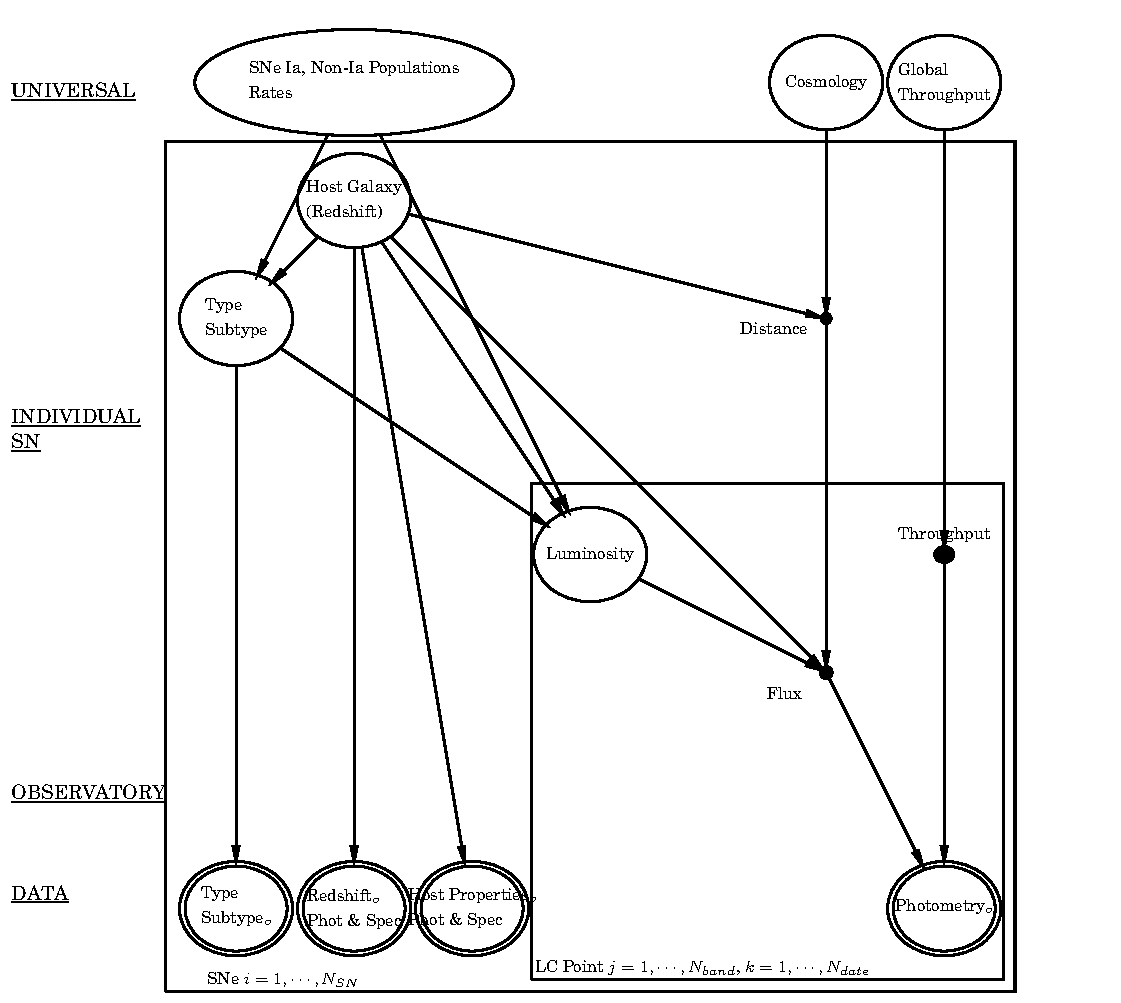
\includegraphics[width=7in]{../results/hdpgm.pdf} 
   \caption{Probabilistic Graphical Model for the SN~Ia analysis.  
   The forward modeling
   flow goes from left to right, starting with the description of the universe, observatory,
   and data.    A transient has host galaxy $g_i$, which determines its redshift $z_i$
   and galaxy parameters $\theta_{gi}$.
   A model with parameters $\theta_\mu$ fix the distance modulus $\mu_i$.
   The transient type $T$ depends on the host-galaxy parameters  $\theta_{gi}$
   and rates $\theta_r$.   The transient
   parameters $\theta_T^X$, $\theta_{Ti}^X$ (and perhaps the host galaxy) determine the luminosity $L$.       The 
   incoming photon flux $n$, $n_g$  are then fixed
   with redshift and distance modulus.
   The instrumental transmission function $\phi$ is calibrated with data ${Z}$ and
   gives the expected
   counts $\overline{\mathit{ADU}}$, $\overline{\mathit{ADU}}_g$. 
   The transient has realized light curves (${ADU}$) and passes selection criteria
   through $\tau_i$ to be included in the sample.  Some transients have spectral data
   ${X}_S$.  The properties of the galaxy identified as the host galaxy is $\theta_G$. 
   \label{pgm:fig}}
\end{figure}

From these fundamental parameters we can determine the expected
signals
through a series of intermediary parameters,
some of which are deterministic (points in Figure~\ref{pgm:fig}) and others
probabilistic (ovals).
\begin{itemize}
\item $z_i$, $\theta_{gi}$ are the galaxy redshift and parameters (e.g.\ mass, sSFR, metallicity).
Each galaxy $g_i$ has its values for these quantities.
\item $\mu_i=\mu(z_i; \theta_\mu)$.  The distance modulus is a function of redshift,
Unspecified at the moment,  it could
be a $\Lambda$CDM prediction with cosmological parameters, a spline with knot values
as parameters.
The redshift of the galaxy is used in the Hubble diagram, peculiar velocities are not considered.
\item $P(T_i | \theta_r, \theta_{gi})$.  The transient type $T_i$, SN~Ia or non-Ia, depends
on the relative rates given the host properties.
\item $P(L_i(t,\lambda)| T_i, \theta_T^{Ia}, \theta_{Ti}^{Ia}, \theta_T^{\mathit{non-Ia}}, \theta_{Ti}^{\mathit{non-Ia}},
\theta_{gi})$.  The source model determines
the luminosity; the model may include intrinsic dispersion to make the luminosity
probabilistic. The  model includes  information on the
source and line-of-sight effects, which specify the effective SED.   Only the
parameters of the model of the appropriate type $T$ are relevant.  The galaxy parameters
$\theta_{gi}$ are included if correlations with host-galaxy properties are to be modeled.
\item $n_i(t,\lambda; L_i, \mu_i, z_i)$, $n_{gi}(t; g_i, \mu_i, z_i)$.  The  fluxes of
the transient and host that are incident at Earth
are fixed by the luminosity, distance modulus, and redshift.
The supernova redshift is required for this calculation,
for simplicity the supernova and host-galaxy redshift are assumed to be equal.
\item $\overline{\mathit{ADU}}$ and
$\overline{\mathit{ADU}}_g$ are the expected counts of the transient and galaxy respectively,
coming from $\int n_i \phi d\lambda$.  
\end{itemize}

The observations are as follows:
\begin{itemize}
\item ${\mathit{ADU}}$ is the realized flux.  It depends on the underlying flux and
the photometric noise.
\item $\theta_G$ represents the galaxy parameters of the
galaxy catalog used to identify prospective host galaxies.
\item ${T}_S$, ${z}_S$, ${\theta}_S$ are the transient type, redshift and properties from
spectroscopic data. Details of the actual measurement are ignored and a direct association
is made with the fluxes of the transient and underlying galaxy $n$, $n_g$.
\item $\tau$ is the score used to decide if the transient is used in the analysis.  It is
determined based on other measurements $\tau(\mathit{ADU},T_S)$.
\item ${Z}$ represents the calibration measurements.   Although this may be given
by the Calibration Task Force, the PGM is written for the more general case where the calibration
is modeled within our analysis.
\end{itemize}

%The likelihood for the model is
%\begin{multline}
%p(\mathit{ADU}, {{T}}_S,{{z}}_S,
%{{\theta}}_S, \theta_G, \tau, Z | g, \theta_\mu, \theta_r, \theta_T^{Ia}, \theta_{Ti}^{Ia}, \theta_T^{non-Ia}, \theta_{Ti}^{non-Ia}, \phi) = \\
%p(\theta_G|g)p(Z|\phi)p(\mathit{ADU}, {{T}}_S,{{z}}_S,
%{{\theta}}_S, \tau | g, \theta_\mu, \theta_r, \theta_T^{Ia}, \theta_{Ti}^{Ia}, \theta_T^{non-Ia}, \theta_{Ti}^{non-Ia}, \phi).
%\label{likelihood:eqn}
%\end{multline}

\section{Simple Example}
\subsection{Model}
\label{example:sec}
A simplified version of the above model,
\begin{equation}
p(\mathit{ADU}, {{T}}_S,{{z}}_S, \theta_G|  \Omega_M, w, \theta_r,\alpha_{Ia},\sigma_{Ia}, \alpha_{\mathit{non-Ia}},\sigma_{\mathit{non-Ia}}),
\end{equation}
is examined in this section and is sketched in Figure~\ref{toypgm:fig}.
The measurements are
\begin{itemize}
\item $\mathit{ADU}$: the measured counts at peak brightness;
\item ${{T}}_S$, ${{z}}_S$: the spectroscopic type and redshift for a subset of transients;
\item $\theta_{G1}$, $\theta_{G2}$: the redshifts of the identified host and neighbor
galaxies.
\end{itemize}
The model parameters are
\begin{itemize}
\item $\Omega_M$, $w$: the parameters of a flat dark-energy cosmology;
\item $\theta_{r1}$, $\theta_{r2}$:  for two redshifts the fraction of transients that are SN~Ia;
\item $\alpha_{Ia}$, $\sigma_{Ia}$, $\alpha_{\mathit{non-Ia}}$, $\sigma_{\mathit{non-Ia}}$:
the luminosity (times $4\pi$) and intrinsic dispersion for SNe~Ia and non-Ia at peak.
Light-curve shape and color are not considered in this simple model.
\end{itemize}

\begin{figure}[htbp] %  figure placement: here, top, bottom, or page
   \centering
   \includegraphics[width=5in]{../results/toy_pgm.pdf} 
   \caption{Probabilistic Graphical Model for the simple SN~Ia analysis. The
   parameters include the cosmological parameters $\Omega_M$ and $w$,
   the luminosities $\alpha$ and intrinsic dispersions $\sigma$ of SNe~Ia and non-Ia's,
   and the relative rate parameters $\theta_{r1}$ and $\theta_{r2}$.  Latent parameters
   include the type $T$ and redshifts of the host and neighboring galaxies $z$ and $z_N$
   for each transient.  The  parameters for distance modulus $\mu$ and
   luminosity $L$ are fixed by the other parameters.  The observables include the measured
   flux $\mathit{ADU}$, spectroscopic type and redshift $T_S$ and $z_S$, and
   the inferred host and neighbor redshifts $\theta_{G1}$ and $\theta_{G2}$.
   \label{toypgm:fig}}
\end{figure}

There are latent model parameters for each transient used internally
by the model:
\begin{itemize}
\item $z$: the cosmological redshifts.
\item $T$: the type, SN~Ia or non-Ia.
\end{itemize}

The transients are divided into samples defined by available data: {\it obs} are transients observed spectroscopically while active, from which $T_S=1$ are those typed
as SN~Ia and $T_S=0$ as non-Ia.  {\it mis} transients are not observed
spectroscopically when active.  The  {\it obs} and {\it mis} samples
are assumed to be drawn from the same underlying distribution, so that 
same SN~Ia and non-Ia parameters apply for both sets.

\subsubsection{Model for the {\it obs} set data}
The modeling of data from the {\it obs} set, which has
spectroscopic observations $T_S$ and redshift
$z_S$, is described as follows.  We are interested in
\begin{align}
p(\mathit{ADU}, {{T}}_S,{{z}}_S|  \Omega_M, w, \theta_r,\alpha_{Ia},\sigma_{Ia}, \alpha_{\mathit{non-Ia}},\sigma_{\mathit{non-Ia}})  &=\sum_T \int_z dz\,
p(\mathit{ADU}, {{T}}_S,{{z}}_S, T, z| \ldots)\\
&= \sum_T \int_z dz\,
p(\mathit{ADU}, {{T}}_S,{{z}}_S| T, z,\dots) p(T,z | \ldots)
\end{align}

A direct association of spectroscopic redshift and type are made so that
\begin{align}
p(z_S|z) &= \delta(z_S-z)\\
p(T_S|T) &= \delta(T_S-T),
\label{specz:eqn}
\end{align}
so that
\begin{align}
p(\mathit{ADU}, {{T}}_S,{{z}}_S|  \ldots) &= 
p(\mathit{ADU}| T=T_S, z=z_s,\dots) P(T_S| z= z_S , \ldots) p(z_S|\ldots).
\label{obs:eqn}
\end{align}
We remark that in a flux limited survey, the pdf's for the data are truncated versions of the universal
pdf's of the observables.

The first term describes the expected counts. Given the redshift
and transient type, the brightness of the underlying population
is modeled as being drawn from a standard candle
with luminosity $4\pi\alpha_X$ and intrinsic magnitude dispersion  $\sigma_X$:
\begin{equation}
\mathit{ADU}| T_S, z_S, \Omega_M, w, \theta_r, \alpha_{Ia},\sigma_{Ia}, \alpha_{\mathit{non-Ia}},\sigma_{\mathit{non-Ia}} \sim \mathcal{N}_{\ln}\left(\ln{\left(\frac{\alpha_{T_S}}{d_L^2(z_S;\Omega_M, w)}\right)}, \frac{\ln{10}}{2.5}\sigma_{T_S}\right),
\end{equation}
where $\mathcal{N}_{\ln}$ is the log-normal distribution and $d_L$ is the luminosity distance.

The subset of objects that enters our analysis comes from a truncated distribution:
\begin{itemize}
\item For transients in set $T_S=1$:
\begin{equation}
\mathit{ADU} | T_S=1, z_S, \Omega_M, w, \alpha_{Ia},\sigma_{Ia} \sim
\frac{\mathcal{N}_{\ln}\left(\ln{\left(\frac{\alpha_{Ia}}{d_L^2(z_S;\Omega_M, w)}\right)}, \frac{\ln{10}}{2.5}\sigma_{Ia}\right)}{P_{Ia}(\mathit{ADU} > \mathit{ADU}_0)}.
\label{adusnIa:eqn}
\end{equation}
\item For transients in set $T_S=0$:
\begin{equation}
\mathit{ADU} | T_S=0, z_S, \Omega_M, w, \alpha_{\mathit{non-Ia}},\sigma_{\mathit{non-Ia}}\sim 
\frac{\mathcal{N}_{\ln}\left(\ln{\left(\frac{\alpha_{\mathit{non-Ia}}}{d_L^2(z_S;\Omega_M, w)}\right)}, \frac{\ln{10}}{2.5}\sigma_{\mathit{non-Ia}}\right)}{P_{non-Ia}(\mathit{ADU} > \mathit{ADU}_0)},
\label{adunonIa:eqn}
\end{equation}
\end{itemize}
where the normalization factor is the complementary cumulative distribution function
for the corresponding log-normal distribution.
It is understood that $p(\mathit{ADU}<\mathit{ADU}_0)=0$ is never evaluated.

The second term gives the type probability. In our model,
the underlying relative rates between SNe~Ia and non-Ia is linear in redshift,
 parameterized by the
its value at $z=0$ and $1.1 \times z_{max}$, 
\begin{equation}
\hat{\theta}_{r}=\theta_{r0}+z\left(\frac{\theta_{r1}-\theta_{r0}}{1.1 \times z_{max}}\right).
\end{equation}
The relative rate for SN~Ia discovery for the truncated distribution is
\begin{equation}
\theta_{r}=\frac{\hat{\theta}_{r}P_{Ia}(\mathit{ADU} > \mathit{ADU}_0)}{\hat{\theta}_{r}P_{Ia}(\mathit{ADU} > \mathit{ADU}_0) + (1-\hat{\theta}_{r})P_{non-Ia}(\mathit{ADU} > \mathit{ADU}_0)}.
\end{equation}
The spectroscopic classifications are drawn from
\begin{equation}
T_S | \Omega_M, w, \theta_{r0}, \theta_{r1} , \alpha_{Ia},\sigma_{Ia}, \alpha_{\mathit{non-Ia}},\sigma_{\mathit{non-Ia}} \sim \text{Bernoulli}(\theta_r).
\end{equation}
Although the underlying type distribution depends only on $ \theta_{r0}$ and $ \theta_{r1}$,  
the observed truncated distribution does depend on the other parameters through 
$P_{X}(\mathit{ADU} > \mathit{ADU}_0)$.

The third term is the redshift distribution of transient discoveries.
In our model we adopt
a redshift distribution of transients in the universe
\begin{equation}
P(z) \propto z^2.
\end{equation}
The redshift distribution of discovered transients is then
\begin{equation}
P(z) = \left(\int_{z_{min}}^{z_{max}} dz'\, z'^2\left( 
\hat{\theta}_{r}P_{Ia}(\mathit{ADU} > \mathit{ADU}_0) + (1-\hat{\theta}_{r})P_{non-Ia}(\mathit{ADU} > \mathit{ADU}_0)
\right)\right)^{-1}z^2.
\end{equation}

In the presented model, the data from different transients are independent.

\subsubsection{Model for the {\it mis} set data}

We now consider the modeling of data from the  {\it mis}
set that has no spectroscopic confirmation.
The redshift measurement is treated as follows:
For each transient there are two galaxies identified as
the potential host, one ($\theta_{G1}$) with high probability $P_{host}$
of being the host and the other
($\theta_{G2}$) at lower $(1-P_{host})$ probability.
In the model, the
true host redshift is $z$ and that of the interloping galaxy is $z_N$.
\begin{equation}
P(\theta_{G1},\theta_{G2}|z, z_N) =
	P_{host}\delta(z-\theta_{G1})\delta(z_N-\theta_{G2}) +
	(1-P_{host}) \delta(z-\theta_{G2})\delta(z_N-\theta_{G1}).
\end{equation}
As for the {\it obs} set, the redshifts of the supernova
 and neighbor are drawn from distributions $P(z) \propto z^2$, $P(z_N) \propto z^2_N$.


The data likelihood is 
\begin{multline}
p(\mathit{ADU}, \theta_{G1}, \theta_{G2} | \Omega_M, w, \theta_r, \alpha_{Ia},\sigma_{Ia}, \alpha_{\mathit{non-Ia}},\sigma_{\mathit{non-Ia}})  \\
= \sum_{T}\int_{z,z_N} dz\,dz_N \, p(\mathit{ADU, \theta_{G1}, \theta_{G2}}| z , z_N, T, \ldots)P(T| z, z_N,\ldots) p(z, z_N|\ldots)\\
 =\sum_{T} \int_{z,z_N} dz\,dz_N\, p(\mathit{ADU}| z ,T, \ldots)p(\theta_{G1}, \theta_{G2}| z , z_N) P(T| z, \ldots) p(z, z_N|\ldots)\\
= \sum_{T} P_{host} p(\mathit{ADU}| z=\theta_{G1} ,T, \ldots) P(T| z=\theta_{G1}, \ldots) p(\theta_{G1},\theta_{G2}|\ldots) \\
 +  (1-P_{host}) p(\mathit{ADU}| z=\theta_{G2} ,T, \ldots) P(T| z=\theta_{G2}, \ldots) p(\theta_{G2},
 \theta_{G1}|\ldots)\\
\propto \sum_{T} P_{host} p(\mathit{ADU}| z=\theta_{G1} ,T, \ldots) P(T| z=\theta_{G1}, \ldots) \\
 +  (1-P_{host}) p(\mathit{ADU}| z=\theta_{G2} ,T, \ldots) P(T| z=\theta_{G2}, \ldots),
\label{adumis:eqn}
\end{multline}
where we take advantage of the fact that
$p(\theta_{G1}, \theta_{G2} | \ldots) = p(\theta_{G2}, \theta_{G1} | \ldots)$ does
not have parameter dependence.

The distribution of $\mathit{ADU}$ for our sample is a truncated version of the
underlying distribution.  
For our analysis, we use the distribution in  Eqn.~\ref{adumis:eqn} normalized by
the complementary cumulative distribution function
\begin{equation}
P(\mathit{ADU}>\mathit{ADU}_0, \theta_{G1}, \theta_{G2}|\ldots) = \int_{\mathit{ADU}_0}^{\infty} p(\mathit{ADU}, \theta_{G1}, \theta_{G2}|\Omega_M, w, \theta_r, \alpha_{Ia},\sigma_{Ia}, \alpha_{\mathit{non-Ia}},\sigma_{\mathit{non-Ia}})d\mathit{ADU}
\end{equation}
for a detection threshold of $\mathit{ADU}_0$.

%I highlight the treatment of redshift in this model; the cosmological redshift
%$z$ is set to the values of the
%observed redshifts through $\delta$-functions.  This choice was made specifically to aid
%in the convergence of the Monte Carlo: the discrete possibilities for redshift allow
%for their marginalized likelihood to be used in the calculation of the posterior.
%A more general model would replace the $\delta$-functions
%with coming from a continuous PDF's.
%Peculiar velocities, redshift measurement errors (particularly from
%photometric redshifts) justify this generalization.
%A transient
%without a spectrum has uncertain type and redshift: the redshift
%of the associated host galaxy, and redshifts expected based on the
%flux of the SN~Ia and non-Ia standard candles,
%are viable but disjoint possibilities for the posterior of
%the true underlying redshift. My runs of this scenario produce chains
%that do not mix so I resorted to the simplified treatment presented here.

\subsection{Analysis of Simulated Data}
The simulation of data from the model presented in \S\ref{example:sec}
and their analysis is implemented in Python and are available
on GitHub\footnote{\url{git@github.com:AlexGKim/abc.git}}.

The results that follow are based on the parameter
choices:
\begin{itemize}
\item Cosmological parameters $\Omega_M=0.28$, $w=-1$.
\item Type~Ia supernovae with intrinsic dispersion $\sigma_{SNIa}=0.1$.
\item Non-Ia supernovae 2 magnitudes fainter than SNe~Ia with intrinsic
dispersion $\sigma_{non-Ia}=1$.
\item $\theta_r=r_0 + (r_1-r_0)z/1.54$ for a constant relative fraction of SNe~Ia where $r_1=0.2$,
$r_0=0.95$.
\item 2000 transients distributed by co-moving volume in the range $0.1<z<1.4$.
\item Detection threshold at approximately the mean brightness SN~Ia at $z=1$.
\item $z_{min}=0.1/1.1$ and $z_{max}=1.4\times 1.1$ is the range of possible misassigned
host redshift.
\item $P_{host}=0.98$ for the probability of correct host-galaxy assignment.
\item Accumulated spectra for 0\%, 20\%, 60\%, and 100\% of discovered transients.
\end{itemize}
This setup is referred to as Model 1.

The Hubble diagram for a realization drawn from this model is shown in Figure~\ref{hd:fig}.
Type~Ia's are shown in blue and non-Ia's in red, those that fall below detection threshold
are faded.  The solid points
represent those objects spectroscopically typed for the case of 20\% follow-up.
The green X's represent the 2\% among those without spectroscopy that
are assigned an incorrect redshift.
%
%\begin{figure}[htbp] %  figure placement: here, top, bottom, or page
%   \centering
%   \includegraphics[scale=0.4]{/Users/akim/project/abc/doc/seed2.pdf}
%   \includegraphics[scale=0.4]{/Users/akim/project/abc/doc/seed2_pop2.pdf}  
%\caption{Hubble diagrams for a realization drawn from the baseline Model 1 (left)
%and Model 2 with a second non-Ia population (right).
%Type~Ia's are shown in blue and non-Ia's in red, those that fall below detection threshold
%are faded.  The green X's represent the 2\% among those without spectroscopy that
%are assigned an incorrect redshift.
%   \label{hd:fig}}
%\end{figure}

The simulated data are analyzed using 
\citet{stan-software:2015},
a probabilistic programming language for
inference of Bayesian models with Hamiltonian Monte Carlo.
In addition to the simulated data,
supplemental priors are applied to the SN~Ia absolute magnitude and intrinsic dispersion
\begin{align}
\alpha_{SNIa} & \sim \mathcal{N}_{\ln}\left(\ln\left(\alpha^0_{SNIa}\right),\frac{\ln{10}}{2.5}0.02\right)\\
\sigma_{SNIa} & \sim \mathcal{N}_{\ln}\left(\ln\left(0.1\right),0.1\right),
\end{align}
where $\alpha^0_{SNIa}$ is the true input luminosity.  This prior is added in lieu of
a pure large SN~Ia sample at low-redshift.

The results of the analyses meet expectations.  As the input data and analyses are
based on the same model, the input parameters lie in reasonable position
within the resultant posterior despite the non-trivial appearance of
the Hubble diagram in Figure~\ref{hd:fig}.
The parameter pdf's are shown in Figure~\ref{contour1:fig} for the ideal case of 100\% spectroscopic classification.  The input values for all 7 parameters fall within the 68\%
credible interval.  The same is true for the unideal case of no
spectroscopic classification.  Table~\ref{seed2:tab} lists the modes
of the $w$ distribution for varying spectroscopic coverage: there is no appreciable
bias relative to the statistical uncertainties.

%\begin{figure}[htbp] %  figure placement: here, top, bottom, or page
%   \centering
%   \includegraphics[scale=0.17]{/Users/akim/project/abc/results/seed2/{contour.2000.1.0}.pdf}
%   \includegraphics[scale=0.17]{/Users/akim/project/abc/results/seed2_pop2/{contour.2000.1.0}.pdf} 
%\caption{Probability distribution functions of the model parameters for the case of
% 100\% spectroscopy for Model 1 (left) and Model 2 (right).
%    Solid lines represent the input parameters.  Dashed lines in the
%   histograms are the 0.16 and 0.84 quantiles. 
%   \label{contour1:fig}}
%\end{figure}

\begin{table}
\centering
\begin{tabular}{|c|c|ccc|}
\hline
Fraction Spec&\%-ile & $w$ &$w$ range & $\Delta w$\\ \hline
SN Ia only&&&&\\
$1.00$ & $0.68$ &$-0.97$ & $[-1.076, -0.801]$ & $0.275$ \\
$1.00$& $0.90$ &$-0.97$ & $[-1.166, -0.718]$ & $0.448$ \\
$1.00$ & $0.95$ &$-0.97$ & $[-1.208, -0.682]$ & $0.525$ \\ \hline
Model 1&&&&\\
$1.00$ &$0.68$ &$-1.08$ & $[-1.196, -0.914]$ & $0.281$ \\
$1.00$ &$0.90$ &$-1.08$ & $[-1.292, -0.826]$ & $0.466$ \\
$1.00$ &$0.95$ &$-1.08$ & $[-1.340, -0.784]$ & $0.556$ \\
$0.60$ &$0.68$ &$-1.08$ & $[-1.227, -0.933]$ & $0.293$ \\
$0.60$ &$0.90$ &$-1.08$ & $[-1.331, -0.836]$ & $0.495$ \\
$0.60$ &$0.95$ &$-1.08$ & $[-1.385, -0.787]$ & $0.598$ \\
$0.20$ &$0.68$ &$-1.15$ & $[-1.249, -0.943]$ & $0.305$ \\
$0.20$ &$0.90$ &$-1.15$ & $[-1.354, -0.851]$ & $0.502$ \\
$0.20$ &$0.95$ &$-1.15$ & $[-1.408, -0.810]$ & $0.597$ \\
$0.00$ &$0.68$ &$-1.09$ & $[-1.218, -0.909]$ & $0.309$ \\
$0.00$ &$0.90$ &$-1.09$ & $[-1.320, -0.812]$ & $0.508$ \\
$0.00$ &$0.95$ &$-1.09$ & $[-1.372, -0.770]$ & $0.602$ \\ \hline
Model 2&&&&\\
$1.00$ &$0.68$ &$-0.94$ & $[-1.078, -0.804]$ & $0.274$ \\
$1.00$ &$0.90$ &$-0.94$ & $[-1.168, -0.720]$ & $0.447$ \\
$1.00$ &$0.95$ &$-0.94$ & $[-1.214, -0.680]$ & $0.534$ \\
$0.60$ &$0.68$ &$-1.09$ & $[-1.182, -0.883]$ & $0.298$ \\
$0.60$ &$0.90$ &$-1.09$ & $[-1.285, -0.791]$ & $0.494$ \\
$0.60$ &$0.95$ &$-1.09$ & $[-1.332, -0.749]$ & $0.583$ \\
$0.20$ &$0.68$ &$-1.09$ & $[-1.247, -0.936]$ & $0.311$ \\
$0.20$ &$0.90$ &$-1.09$ & $[-1.359, -0.840]$ & $0.518$ \\
$0.20$ &$0.95$ &$-1.09$ & $[-1.413, -0.798]$ & $0.614$ \\
$0.00$ &$0.68$ &$-1.11$ & $[-1.266, -0.948]$ & $0.317$ \\
$0.00$ &$0.90$ &$-1.11$ & $[-1.375, -0.850]$ & $0.525$ \\
$0.00$ &$0.95$ &$-1.11$ & $[-1.428, -0.808]$ & $0.621$ \\
\hline
\end{tabular}
\caption{Mode and credible intervals of $w$ for only the SNe~Ia, Model 1, and Model 2 for varying
fractions of spectroscopic coverage. \label{seed2:tab}}
\end{table}

%\begin{figure}[htbp] %  figure placement: here, top, bottom, or page
%   \centering
%   \includegraphics[scale=0.17]{/Users/akim/project/abc/results/seed2/{contour.2000.0.0}.pdf}
%   \includegraphics[scale=0.17]{/Users/akim/project/abc/results/seed2_pop2/{contour.2000.0.0}.pdf} 
%\caption{Probability distribution functions for the difference in parameters
%with 100\% and 0\% spectroscopic folowup for Model 1 (left) and Model 2 (right).  \label{contour2:fig}}
%\end{figure}

Though the decrease in spectroscopic coverage produces low bias, it does lead to
increased parameter uncertainties.
The credible intervals for $w$ are shown in Table~\ref{seed2:tab}:
for the case of 100\% follow-up the range of the 68\% $w$ interval is $\Delta w = 0.281$. 
At the opposite extreme of no spectroscopic classification the $w$ interval inflates to
$\Delta w = 0.309$, a constraining result nevertheless considering that none of the
objects are directly typed and redshifted.





As a stress test, we generate a simulated data based on a different model
referred to as Model 2, which
has a second non-Ia population with average luminosity 0.5 mag fainter
than the Ia's and 0.25 mag dispersion.
The relative rates of the original non-Ia population relative to the second is quadratic:
\begin{equation}
1 -\frac{0.8}{1.54}z^2.
\end{equation}
A realization of transients from this model, using the same random seeds
as Model 1, is shown in Figure~\ref{hd:fig}.

When there is 100\% spectroscopic coverage the   $\Omega_M$--$w$  posterior accommodates the input 
parameters, as shown  in
Figure~\ref{contour1:fig}.
A salient feature that contrasts with Model 1 is 
seen in the modes for $w$ listed in Table~\ref{seed2:tab}: biases
larger than the statistical uncertainties appear with decreasing
spectroscopic coverage.  Note that the Hubble diagrams
in these analyses are almost identical: there are redshift misassignments
for 2\% of the transients that lack spectroscopy. 


%\begin{figure}[htbp] %  figure placement: here, top, bottom, or page
%   \centering
%   \includegraphics[scale=0.35]{/Users/akim/project/abc/results/seed2_pop2/{contour.2000.1.0}.pdf} \newline
%\caption{Probability distribution function for $\Omega_M$--$w$,
% 100\% spectroscopy, biased.
%    Solid lines represent the input cosmology.  Dashed lines in the
%   histograms are the 0.16 and 0.84 quantiles. 
%   \label{contour3:fig}}
%\end{figure}
%
%\begin{figure}[htbp] %  figure placement: here, top, bottom, or page
%   \centering
%   \includegraphics[scale=0.35]{/Users/akim/project/abc/results/seed2_pop2/{contour.2000.0.0}.pdf} \newline
%\caption{Probability distribution function for $\Omega_M$--$w$,
% no spectroscopy, biased.
%   \label{contour4:fig}}
%\end{figure}


Some initial conclusions.
\begin{itemize}
\item Knowing the underlying model that produces data, you should
get results statistically consistent with the truth.  A tautology?
\item Typing is important when the non-Ia model is not accurate.
\end{itemize}

%
%\subsubsection{SN~Ia Only}
%A classical analysis would only include confirmed SNe~Ia with a definitive
%redshift. The realization of simulated data has 415 Type~Ia supernovae.
%Results of the analysis of a pure SN~Ia sample with no
%host misclassification are presented:  Figure~\ref{contour.ia_only:fig}
%shows the posteriors for  $\Omega_M$--$w$ and Table~\ref{ia_only:tab} the
%credible equal-tailed intervals for $w$.  The true $w=-1$ is within
%the 0.58 credible interval. (Note that $w$ is the parameter
%of most interest for the experiment.)
%
%\begin{figure}[htbp] %  figure placement: here, top, bottom, or page
%   \centering
%   \includegraphics[scale=0.55]{/Users/akim/project/abc/results/{contour..ia_only.500}.pdf} \newline
%\caption{Probability distribution function for $\Omega_M$--$w$ for only SNe~Ia
%   all with spectra.
%   Solid lines represent the input cosmology.  Dashed lines in the
%   histograms are the 0.16 and 0.86 quantiles. 
%   \label{contour.ia_only:fig}}
%\end{figure}
%
%\begin{table}
%\centering
%\begin{tabular}{|c|cc|}
%\hline
%\%-ile & $w$ range & $\Delta w$\\ \hline
%$0.68$ & $[-1.254, -0.975]$ & $0.279$ \\
%$0.90$ & $[-1.347, -0.889]$ & $0.458$ \\
%$0.95$ & $[-1.396, -0.846]$ & $0.550$ \\
%\hline
%\end{tabular}
%\caption{Credible intervals of $w$ using the SNe~Ia only with spectroscopic
%observations.\label{ia_only:tab}}
%\end{table}
%
%\subsubsection{Full Sample: Varying Spectroscopic Completeness}
%We now turn to the full sample of SNe~Ia and non-Ia's.  Recall that our simple
%model treats the non-Ia's in the sample
%as standard candles with a large (1 mag) intrinsic dispersion.
%
%Results for the $\Omega_M$--$w$ posterior for the
%case of 40\%, 70\%, and 100\% spectroscopic completeness
%are shown in Figures~\ref{contour.200:fig}, \ref{contour.350:fig}, and
%\ref{contour.500:fig} respectively.
%The credible intervals
%of $w$ for are given in Table~\ref{compare:tab}, with
%the input $w=-1$ within the 0.65, 0.49, and 0.47  intervals
%respectively.
%
%\begin{figure}[htbp] %  figure placement: here, top, bottom, or page
%   \centering
%   \includegraphics[scale=0.40]{/Users/akim/project/abc/results/{contour.200}.pdf} 
%   \caption{Probability distribution function for $\Omega_M$--$w$ for:
%    SNe~Ia and non-Ia with 40\%  spectroscopic completeness.
%   \label{contour.200:fig}}
%\end{figure}
%
%\begin{figure}[htbp] %  figure placement: here, top, bottom, or page
%   \centering
%   \includegraphics[scale=0.40]{/Users/akim/project/abc/results/{contour.350}.pdf} 
%   \caption{Probability distribution function for $\Omega_M$--$w$ for
%    SNe~Ia and non-Ia with 70\%  spectroscopic completeness.
%   \label{contour.350:fig}}
%\end{figure}
%
%\begin{figure}[htbp] %  figure placement: here, top, bottom, or page
%   \centering
%   \includegraphics[scale=0.40]{/Users/akim/project/abc/results/{contour.500}.pdf} 
%   %\includegraphics[scale=0.55]{/Users/akim/project/abc/results/{contour.200}.pdf}    
%   \caption{Probability distribution function for $\Omega_M$--$w$ for
%    SNe~Ia and non-Ia with 100\%  spectroscopic completeness.
%   \label{contour.500:fig}}
%\end{figure}
%
%\begin{table}[htbp] 
%\centering
%\begin{tabular}{|cc|cc|}
%\hline
%\# Spectra & \%-ile & $w$ range & $\Delta$\\ \hline
%200& $0.68$ & $[-1.284, -0.991]$ & $0.293$ \\
%200& $0.90$ & $[-1.385, -0.900]$ & $0.485$ \\
%200& $0.95$ & $[-1.435, -0.860]$ & $0.575$ \\
%350& $0.68$ & $[-1.243, -0.952]$ & $0.291$ \\
%350& $0.90$ & $[-1.339, -0.858]$ & $0.481$ \\
%350& $0.95$ & $[-1.390, -0.817]$ & $0.573$ \\
%500& $0.68$ & $[-1.236, -0.948]$ & $0.289$ \\
%500& $0.90$ & $[-1.336, -0.861]$ & $0.475$ \\
%500& $0.95$ & $[-1.385, -0.815]$ & $0.570$ \\
%\hline
%\end{tabular}
%\caption{Credible intervals of $w$ given different levels of spectroscopy.  \label{compare:tab}}
%\end{table}
%
%As would be expected, the better the spectroscopic completeness, the less bias
%and smaller uncertainties that are obtained.
%
%
%\section{Subsections of the Model}
%
%\subsection{Type}
%\label{type:sec}
%Since our transient sample may not consist purely of SNe~Ia, the model
%has a term of the form $P(T, G | z,\mu)$, which should account for all types of
%objects that could potentially be mistaken for Type~Ia:
%the rates and association with host galaxies are described for
%the full population of potential interlopers.
%This term is not currently well known, particularly at the highest redshifts probed by DES.
%
%An idea is to consider two types: SN~Ia and non-SN~Ia, where the latter's
%intrinsic distributions have loose priors.  Transients that have been spectroscopically
%classified as non-Ia will provide the strongest leverage in constraining the
%contamination: this subset must be unbiased or properly weighted
%relative to the underlying population that constitutes the Hubble diagram.
%Running the model on a pure sample of SNe~Ia can have benefits.
%As discussed in \S\ref{systematics:sec}, comparing these results with
%those from the full sample provides
%a test of systematics.  Alternatively, the non-Ia model may be better constrained
%with the pure sample.
%
%
%To minimize the contribution of non-Ia contamination we strive for
%a pure sample selection so that $P(T=\text{non-Ia}| \mu) \rightarrow 0$.
%
%
%\subsection{Host Matching}
%\sloppy
%The host-galaxy properties depend on the GC and the transient
%coordinates $P({z}_H, {\theta}_H | {\mathit{Gals.}}, \text{RA/Dec})$.  With a
%spectrum of the transient and the underlying background, identification of the host galaxy
%is usually straightforward.
%Otherwise, projections or ambiguous cases can result in the misidentification of
%the host.
%Other supernova surveys (e.g.\ SNLS) 
%with spectroscopically confirmed host associations (e.g.\ with
%matched transient and galaxy redshifts) that replicate the DES population
%can be used to put a prior on this probability.
%
%%An effective way of addressing this term is to
%%analyze the supernovae assuming a correct host match, and
%%experimentally determine $P(\text{mismatch} )$ and
%%$\left. \langle {\mu}-\mu(z)\rangle \right|_{\text{mismatch}}$, $\left. \langle {z}-z \rangle \right|_{\text{mismatch}}$ and cross-terms to correct bias in the Hubble diagram. 
%
%
%% only model $T=\text{SN~Ia}$,
%%and experimentally determine $P(\text{non-Ia})$, 
%%$\left. \langle \mu-\mu_{model} \rangle \right|_{non-Ia}$, and its uncertainty for the
%%sample of non-Ia's that are discovered and misclassified as SN~Ia.
%%This measurement is achieved through spectroscopic
%%typing of a subset drawn from the populations used in the Hubble diagram.
%%The weighted bias would be added as a correction to the Hubble diagram under the assumption that all objects are SNe~Ia.
%
%
%\section{Systematic Tests}
%\label{systematics:sec}
%The Hubble diagrams of subsets of data quantify systematic uncertainty.  
%Subsets that may be expected to show evidence for systematics include:
%spectroscopically typed SNe~Ia; transients in deep (3) versus shallow (1/2) DES fields;
%transients with NIR data; splits based on host properties.
%
%A potentially more probative test is to compare the distance moduii inferred for the same
%supernovae, but reducing the amount of data considered.  A subset of DES
%transients have higher signal-to-noise, spectroscopic confirmation, and NIR coverage than
%the average transient, we can take away that extra information in calculating distance modulus
%to get $P(\mu | \mathit{data} - \mu | \mathit{data}^-, z | \mathit{data} - z | \mathit{data}^-)$.
%It is possible that differences in $\mu$s and $z$s have smaller uncertainties that the
%$\mu$ and $z$ alone due to common measurement uncertainties. 
%
%
%
%Generically ${{T}}$ can describe sample selection.  I choose to focus
%on objects typed as SN~Ia, rather than  all discovered transients, not just those typed as SN~Ia. 
%The non-Ia transient population has significant model uncertainty and the information they impart on the expansion history is weak:  I anticipate it is cleaner to limit ourselves to
%modeling discoveries we think are SN~Ia. This restriction does not obviate the need
%to consider non-Ia contamination in the sample, rather
%we only need to model non-Ia's
%that are mistaken for Ia and not all discovered transients. 

\bibliography{/Users/akim/Documents/alex}

\end{document}

